\begin{figure*}
    \centering
    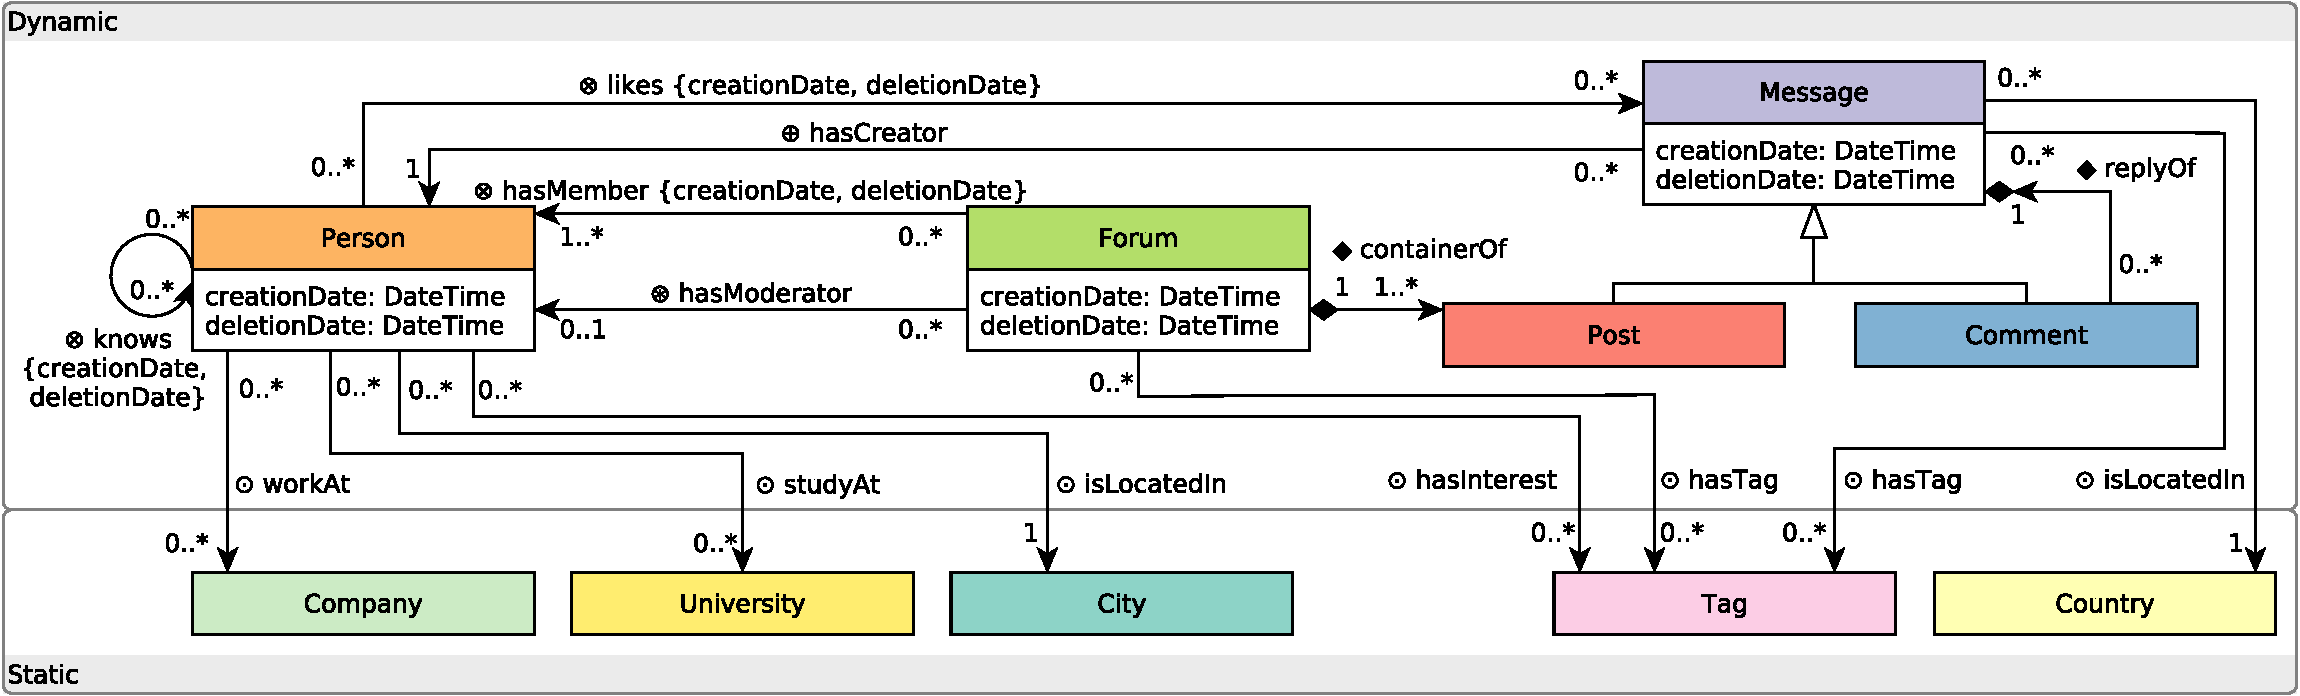
\includegraphics[width=0.95\linewidth]{figures/schema-compact.pdf}
    \caption{%
    Partial LDBC social network schema depicted using a UML-like notation,
    focusing on the dynamic part of the graph (non-lifespan attributes and irrelevant entity types in the static part are omitted).
    %Only lifespan attributes (creation and deletion dates) are shown, other attributes are omitted. %(e.g. Person's first name, birthday, etc.)
    In the dynamic part of the graph,
    all \emph{node types} and
    all $\otimes$~\emph{edge types with many-to-many cardinality between two dynamic node types} have individual lifespan attributes.
    The {\Large $\filleddiamond$}~\emph{containment edges} get their lifespan attributes from the contained endpoint (whose lifespan attributes are constrained by the container endpoint).
    $\oplus$~\tHasCreator follows the semantics of containment edges (even though it does not express an explicit containment relation).
    $\oast$~\tHasModerator is a one-to-many edge that is treated separately depending on the \tForum category (see \autoref{sec:hasModerator}).
    The $\odot$~\emph{edges between a dynamic and a static node} get their lifespan attributes from their dynamic endpoint.
    }
    \label{fig:schema}
\end{figure*}